% ICEIR 2026 -- Springer LNNS (llncs class). Compile on Overleaf with pdfLaTeX.
% Results: code/results/iceir/ (code/src/rerun_iceir.py, code/src/review_iceir.py); figure: make_figures.py
\documentclass[runningheads]{llncs}
\usepackage[T1]{fontenc}
\usepackage[utf8]{inputenc}
\usepackage{graphicx}
\usepackage{cite}
\usepackage{microtype}
\usepackage{booktabs}
\usepackage{amsmath,amssymb}
\usepackage{array}
\usepackage{tikz}
\usetikzlibrary{arrows.meta,positioning}
\usepackage[hidelinks]{hyperref}
\graphicspath{{figures/}}
\providecommand{\doi}[1]{\url{https://doi.org/#1}}

\begin{document}
\setlength{\emergencystretch}{1.5em}

\title{Reproducing or Predicting? Regulation-Grounded Evaluation of Debt-Group Classification and Early Warning in a Vietnamese Commercial Bank}
\titlerunning{Reproducing or Predicting Debt-Group Migration?}

\author{Le Thi Thanh An\inst{1,2} \and
Le Kim Thu\inst{3} \and
Dam Cong Danh\inst{3}\thanks{Corresponding author.}}
\authorrunning{T. T. A. Le, K. T. Le, and C. D. Dam}
\institute{University of Economics and Law, Ho Chi Minh City, Vietnam \and
Vietnam National University, Ho Chi Minh City, Vietnam \and
School of Applied Mathematics and Informatics, Hanoi University of Science and Technology, No.~1 Dai Co Viet, Hanoi, Vietnam\\
\email{danh.dc251317M@sis.hust.edu.vn}}

\maketitle

\begin{abstract}
Machine-learning models for bank credit risk are often judged by how well they reproduce the current debt group on a random split of one snapshot. Using two consecutive monthly snapshots (April and May 2026; about 100,000 loans each) of a Vietnamese commercial bank, we show what such evaluations hide. First, a regulation-grounded leakage audit finds that off-balance-sheet unpaid interest, which accounting rules make a consequence of the debt group, passes Information Value screening yet inflates five-class Macro-F1 from 0.43 to 0.69; its relation to the group also shifted between extracts, causing 835 group-1 loans to be misclassified as group~4 in May. Second, splitting the out-of-time snapshot by contract overlap shows that apparent temporal stability is partly an artefact: without the interest fields, Macro-F1 is 0.49 on contracts seen in training but 0.40 on unseen ones, and an apparent 13--32\% degradation was traced to a silent date-encoding change between extracts. Third, for 31-day migration to a worse group (0.27\% of loans), 83\% of events are mechanical crossings of the regulation's days-past-due thresholds. A rule ranking loans by their distance to the next threshold reaches an average precision (AP) of 0.20, as high as a gradient-boosting model without overdue fields; adding overdue fields at prediction time doubles AP to 0.39 and raises the share of migrations in the top 1\% of the portfolio from 48\% to 66\%. Non-mechanical migrations remain hard to anticipate, and whether these results hold in later periods remains to be tested.

\keywords{Credit risk \and Early warning \and Data leakage \and Out-of-time validation \and Regulatory baseline \and Recall@k.}
\end{abstract}

% ---------------------------------------------------------------------------
\section{Introduction}
\label{sec:intro}

Vietnamese commercial banks must classify every loan into one of five debt groups of increasing risk, with groups 3--5 constituting non-performing debt. The framework in force is Circular 31/2024/TT-NHNN as amended by Circular 37/2025/TT-NHNN~\cite{sbv2024tt31}, which retains the five-group structure of Circular 11/2021/TT-NHNN~\cite{sbv2021tt11} and sets days-past-due (DPD) thresholds of 10, 90, 180 and 360 days between consecutive groups. The group determines specific provisioning under Decree 86/2024/ND-CP~\cite{gov2024nd86} and interest-income recognition under Decree 135/2025/ND-CP~\cite{gov2025nd135}. Machine learning (ML) is increasingly proposed to support this process, and benchmarking studies consistently place tree ensembles among the strongest methods on tabular credit data~\cite{lessmann2015benchmarking,brown2012experimental}.

Studies of this kind, including several for Vietnamese banks~\cite{tran2021mlcredit,trung2024credit,nguyen2024ews}, typically report accuracy, F1 or the area under the receiver operating characteristic curve (ROC-AUC). When the target is the debt group and evaluation uses a random split of one reporting snapshot, three questions remain open: whether the inputs are admissible given how they are produced, whether an out-of-time (OOT) test truly measures performance on unseen loans, and whether a model predicts more than the regulation's own DPD thresholds already imply. We examine them on two consecutive monthly snapshots of a Vietnamese commercial bank (100,617 and 100,274 contracts). The contributions are:

\begin{itemize}
\item[\textbf{C1}] A \emph{regulation-grounded leakage audit}, with a field-level register (Appendix~\ref{app:register}). A field with an Information Value (IV) of about zero is shown to be a consequence of the label under Decree 135/2025/ND-CP; it inflates five-class Macro-F1 from 0.43 to 0.69, and its shifting relation to the label causes systematic out-of-time errors.
\item[\textbf{C2}] An \emph{overlap-aware out-of-time evaluation} that separates next-month contracts seen in training from unseen ones, showing that the usual OOT figure overstates temporal transfer, together with between-extract integrity checks that exposed a silent date-encoding change producing a spurious 13--32\% decline.
\item[\textbf{C3}] \emph{Regulatory baselines for early warning evaluated as budget-constrained retrieval}: debt-group migration is decomposed into mechanical DPD-threshold crossings and other events, and ML models are compared with a distance-to-threshold rule, a scorecard and a learning-to-rank objective using fold-level Recall@k, average precision (AP), severity-weighted NDCG, dependence-corrected tests and a provision-weighted choice of the review budget.
\end{itemize}

\paragraph{Relation to our prior work.} An earlier paper by the same authors~\cite{an2026sebl}, presented at the UEL SEBL 2026 conference on 6 October 2026, used a different extract from the same bank: one undated snapshot of 27,001 contracts with 21 columns from around 2020. It addressed only five-class classification, with a random split, class weighting and an empirical diagnostic of one date variable. The present paper uses two dated 2026 snapshots with 33 columns, adds the migration task, an overlap-aware OOT test and regulatory baselines, and grounds leakage decisions in accounting regulation; no table, figure or numerical result from~\cite{an2026sebl} is reused.

Section~\ref{sec:related} reviews related work and the research gap, Section~\ref{sec:data} defines the data and tasks, Section~\ref{sec:method} the methodology, Section~\ref{sec:results} the results, Section~\ref{sec:discussion} the implications, and Section~\ref{sec:conclusion} concludes.

% ---------------------------------------------------------------------------
\section{Related Work}
\label{sec:related}

\subsection{Machine Learning for Credit Scoring}

Large benchmarks~\cite{baesens2003benchmarking,lessmann2015benchmarking} find that ensembles perform well on average but that rankings depend on the dataset and metric, and the best algorithm changes with class imbalance~\cite{brown2012experimental}. Gradient boosting (XGBoost~\cite{chen2016xgboost}, LightGBM~\cite{ke2017lightgbm}, CatBoost~\cite{prokhorenkova2018catboost}) dominates recent tabular work. In Vietnam, Nguyen and Ngo~\cite{nguyen2025boosting} compare AdaBoost, XGBoost, LightGBM and CatBoost for personal default on 7,542 customers (2014--2022, 12 features) and find LightGBM best. Nguyen et al.~\cite{nguyen2024ews} build an early-warning system for debt-group migration at one bank with logistic regression, support vector machine (SVM), decision tree and random forest: random forest reaches the highest accuracy (81.84\%) for migration into overdue debt, SVM the highest recall (91.48\%, at 46.62\% accuracy), and performance declines on new data. Credit scoring for Vietnamese commercial banks is also studied in~\cite{tran2021mlcredit,trung2024credit}. These studies evaluate binary classifiers at a fixed threshold.

\subsection{Leakage, Dataset Shift and Ranking Evaluation}

Leakage is the use of information not legitimately available at prediction time~\cite{kaufman2012leakage}. In scorecard practice, IV is the standard univariate screen: an IV of 0.3 or more is rated strong~\cite{siddiqi2006credit}, and much higher values (e.g., above 0.5 or 1.0) prompt a leakage check. IV contrasts good and bad loans after binning, so a zero-inflated leaking field can pass unnoticed. Out-of-time samples are the usual safeguard against dataset shift~\cite{siddiqi2006credit,morenotorres2012unifying}. For early warning, Khandani et al.~\cite{khandani2010consumer} forecast consumer delinquency months ahead from transaction and credit-bureau data, and rating-migration studies estimate transition probabilities between grades~\cite{lando2002analyzing}. With rare positives, precision--recall measures such as AP are more informative than ROC analysis~\cite{saito2015precision}. Recall@k, the share of events found in the top $k\%$ of a ranking, equals the capture rate read from the cumulative gains (lift) chart and is the ordinate of the cumulative accuracy profile (CAP) used in scorecard and rating validation~\cite{siddiqi2006credit,engelmann2003testing}; treating a review queue with a fixed budget as retrieval adds rank-sensitive measures that weight its top, such as AP and normalised discounted cumulative gain (NDCG), and learning-to-rank objectives. Comparisons across resampled folds need the variance correction of Nadeau and Bengio~\cite{nadeau2003inference}. SHapley Additive exPlanations (SHAP)~\cite{lundberg2017unified,lundberg2020tree} are widely used to explain credit models~\cite{bussmann2021explainable}.

\subsection{Research Gap}
\label{sec:gap}

\paragraph{G1: leakage is screened statistically, not by provenance.} In Vietnamese bank data several reporting fields, such as specific provisions and off-balance-sheet interest, are \emph{produced} from the debt group by provisioning and accounting rules~\cite{gov2024nd86,gov2025nd135}. To our knowledge, no published study judges input admissibility by the regulatory process that generates each field, and Section~\ref{sec:leak} shows that an IV screen can miss such a field entirely while flagging an innocent one.

\paragraph{G2: out-of-time tests ignore contract overlap.} Consecutive monthly snapshots contain largely the same loans, so a next-month test set overlaps the training data. We are not aware of credit-scoring studies that separate seen from unseen contracts when reporting OOT performance.

\paragraph{G3: early warning lacks regulatory baselines.} Early-warning studies compare ML models with one another at fixed thresholds~\cite{nguyen2024ews}. Because migration between groups is largely defined by DPD thresholds, the relevant benchmark is the ranking already implied by the regulation, evaluated under a review budget. G1--G3 correspond to C1--C3.

% ---------------------------------------------------------------------------
\section{Data and Problem Formulation}
\label{sec:data}

\subsection{Data}

The data are two monthly credit-information extracts of the same bank's loan book, with an identical 33-column schema based on the State Bank of Vietnam reporting template: 30 April 2026 (100,617 contracts) and 31 May 2026 (100,274 contracts). The target is the bank's self-assessed debt group (Table~\ref{tab:dist}). Group~1 is 89 times larger than group~3, but the rare groups remain large enough in absolute terms for per-group evaluation. Of the April contracts, 98,968 also appear in May; 1,306 May contracts are new.

\begin{table}[t]
\centering
\caption{Debt-group distribution in the two snapshots.}
\label{tab:dist}
\small
\begin{tabular}{@{}lrrrrrr@{}}
\toprule
& G1 & G2 & G3 & G4 & G5 & Total\\
\midrule
30/04/2026 & 88,875 & 6,321 & 998 & 1,446 & 2,977 & 100,617\\
\quad share (\%) & 88.33 & 6.28 & 0.99 & 1.44 & 2.96 & 100.00\\
31/05/2026 & 88,527 & 6,339 & 991 & 1,421 & 2,996 & 100,274\\
\quad share (\%) & 88.28 & 6.32 & 0.99 & 1.42 & 2.99 & 100.00\\
\bottomrule
\end{tabular}
\end{table}

\subsection{Two Tasks}

Table~\ref{tab:tasks} defines the two tasks. Task~1 \emph{reproduces} the current group from fields of the same snapshot; Task~2 \emph{predicts} whether loan $i$ moves to a worse group within 31 days, $Y_i=\mathbb{I}(G_{i,T+h}>G_{i,T})$ with $T=$ 30 April 2026 and $h=31$ days, using only fields observed at $T$. All 265 migrations move by exactly one group (214 from group 1 to 2, 10 from 2 to 3, 10 from 3 to 4 and 31 from 4 to 5), so a rule predicting no migration is 99.73\% accurate and the task is treated as ranking a review queue.

\begin{table}[t]
\centering
\caption{The two tasks. OOT: out-of-time; CV: cross-validation; AP: average precision.}
\label{tab:tasks}
\scriptsize
\begin{tabular}{@{}>{\raggedright\arraybackslash}p{1.7cm}>{\raggedright\arraybackslash}p{4.6cm}>{\raggedright\arraybackslash}p{5.3cm}@{}}
\toprule
& Task 1: reproduce the current group & Task 2: predict 31-day migration\\
\midrule
Unit & Contract in a snapshot & Contract present at $T$ and $T+h$ (98,968)\\
Label & Debt group 1--5 (multi-class) & Moves to a worse group by $T+h$ (265 events, 0.27\%)\\
Inputs & 20 admissible fields of the same snapshot (Sect.~\ref{sec:leak}) & The same 20 fields at $T$, plus overdue amounts and DPD at $T$\\
Training / evaluation & 80/20 stratified split of April; all of May as OOT, split by contract overlap & Stratified 5-fold CV repeated 10 times (50 folds)\\
Primary measure & Macro-F1 & AP; Recall@k and Precision@k for a review budget of $k\%$\\
\bottomrule
\end{tabular}
\end{table}

% ---------------------------------------------------------------------------
\section{Methodology}
\label{sec:method}

\begin{figure}[t]
\centering
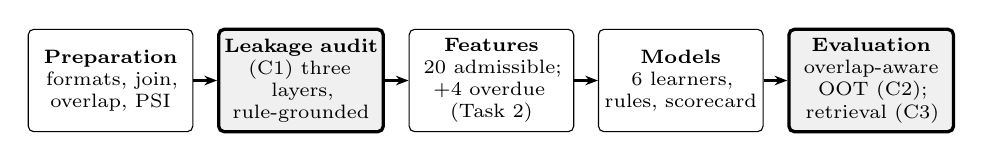
\begin{tikzpicture}[font=\scriptsize, node distance=3mm,
  box/.style={draw, rounded corners=2pt, align=center, text width=1.95cm, minimum height=1.3cm, inner sep=2pt},
  key/.style={box, very thick, fill=gray!12},
  arr/.style={-{Stealth[length=1.6mm]}, thick}]
\node[box] (a) {\textbf{Preparation}\\formats, join,\\overlap, PSI};
\node[key, right=of a] (b) {\textbf{Leakage audit}\\(C1) three layers,\\rule-grounded};
\node[box, right=of b] (c) {\textbf{Features}\\20 admissible;\\+4 overdue (Task 2)};
\node[box, right=of c] (d) {\textbf{Models}\\6 learners,\\rules, scorecard};
\node[key, right=of d] (e) {\textbf{Evaluation}\\overlap-aware OOT (C2);\\retrieval (C3)};
\draw[arr] (a)--(b); \draw[arr] (b)--(c); \draw[arr] (c)--(d); \draw[arr] (d)--(e);
\end{tikzpicture}
\caption{Pipeline. Shaded boxes mark the main contributions. PSI: population stability index.}
\label{fig:pipeline}
\end{figure}

\subsection{Data Preparation and Integrity}
\label{sec:prep}

\paragraph{A silent date-encoding defect.} In our first out-of-time run, every model appeared to deteriorate markedly in May, with relative Macro-F1 declines from 12.7\% (logistic regression) to 32.1\% (CatBoost). The cause was a data defect, not dataset shift: the April extract stores disbursement and contract end dates as \texttt{yyyymmdd} integers, whereas the May extract stored them as Excel serial numbers (e.g., 45965 for 4 November 2025). The parser recognised only the former and, without raising an error, returned empty values for the whole May columns, so the three date-derived features were 100\% missing in the OOT set and were silently imputed with training medians. A between-extract comparison of missing rates exposed the problem. After the dates were standardised to \texttt{yyyymmdd} at source, the apparent degradation disappeared and the median loan age rose from 395 to 426 days, i.e., by one month, as expected; the parser now rejects any other format instead of returning missing values, and all results below use the corrected data.

\paragraph{Joining and partitioning.} Snapshots are joined on the contract key. The 1,649 April contracts absent in May (settled, written off or re-registered; the data do not say which) have no migration label; 97.3\% of them are in group~1, and a sensitivity analysis counts exits from groups 2--5 as events. May contracts are partitioned into those in the April training split (79,144), in the April test split (19,824) and new (1,306). Feature stability between snapshots is measured by the population stability index (PSI); once the three restructuring fields are set to zero for never-restructured loans, no feature has missing values in either snapshot.

\subsection{Regulation-Grounded Leakage Audit (C1)}
\label{sec:leak}

Every field is classified by the process that writes it (Table~\ref{tab:audit}; full register in Appendix~\ref{app:register}).

\begin{table}[t]
\centering
\caption{Three-layer leakage audit of the 33 fields. CIC: National Credit Information Centre.}
\label{tab:audit}
\scriptsize
\begin{tabular}{@{}>{\raggedright\arraybackslash}p{1.9cm}>{\raggedright\arraybackslash}p{4.3cm}>{\raggedright\arraybackslash}p{5.4cm}@{}}
\toprule
Layer & Fields & Decision and basis\\
\midrule
1. Label restatements (7) & CIC-reconciled group; overdue principal and interest amounts and their overdue dates; specific provisions required and booked & Excluded in Task~1: alternative label, direct classification criteria (DPD thresholds~\cite{sbv2024tt31}), or provisions computed from the group (rates 0/5/20/50/100\%~\cite{gov2024nd86}). Overdue fields re-enter Task~2 as states at $T$.\\
2. Identifiers, duplicates, constants (6) & Customer and contract identifiers (4); recovery date ($=$ contract end date); paid amount (always 0) & Excluded: no information\\
3. Rule-grounded review & Off-balance-sheet unpaid interest; on-balance-sheet interest receivable & Recorded by group under Art.~13(2)(a) of Decree 135/2025/ND-CP~\cite{gov2025nd135}; quantified by ablation; excluded from the main Task-1 configuration\\
\bottomrule
\end{tabular}
\end{table}

The Layer-3 evidence is regulatory, not merely statistical. Article~13(2)(a) of Decree 135/2025/ND-CP, in force at both snapshot dates (it superseded Circular 16/2018/TT-BTC and was amended by Decree 316/2026/ND-CP only after them), lets banks recognise accrued interest as revenue only for loans classified as standard; interest on other loans, and on loans kept in the standard group under state policy, is monitored off balance sheet~\cite{gov2025nd135}. Accordingly, off-balance-sheet interest is positive for 0.01\% of group-1 loans but for 21.5\%, 78.1\%, 93.0\% and 97.2\% of groups 2--5 in April. Its IV is about zero, because 93.6\% of its values are zero and decile binning puts nearly all records in one bin; the only field with IV above 1.0 is loan age (1.12), which more plausibly reflects seasoning. The main Task-1 results therefore use the \emph{conservative} configuration without both interest fields; the full configuration measures the inflation due to leakage. In Task~2 the interest and overdue fields describe the state at $T$, before the event, and are admissible provided they are not revised retroactively.

\subsection{Models, Baselines and Evaluation}
\label{sec:eval}

Six learners are compared: logistic regression (LR), decision tree (DT; depth 10), random forest (RF; 300 trees), XGBoost (XGB) and LightGBM (LGBM) (400 trees, learning rate 0.05, depth 6 and 8 respectively) and CatBoost (CB; 400 iterations, with balanced class weights instead of SMOTE because its categorical inputs cannot be interpolated). Hyper-parameters are fixed a priori at common library-style values; a 12-configuration grid is used only as a sensitivity check on the internal test split, and the May snapshot is never used for any choice. Four imbalance strategies are compared (none, class weights, moderate synthetic minority over-sampling (SMOTE)~\cite{chawla2002smote} and both); all preprocessing and resampling are fitted inside each training fold within an \texttt{imblearn} pipeline. Twenty features remain after the audit (12 numeric, 8 categorical, including loan age, days to maturity, actual tenor and a restructuring flag engineered from the dates).

For Task~2, the main models are XGB on the 20 features and XGB with four overdue fields at $T$ (principal and interest DPD and amounts). They are compared with: (i) a rule ranking loans by their distance to the next DPD threshold (10, 91, 181 and 361 days for groups 1--4); (ii) DPD alone; (iii) univariate rankings by each interest field; (iv) a logistic scorecard on weight-of-evidence (WOE) bins~\cite{siddiqi2006credit}; and (v) XGB with a pairwise learning-to-rank objective, with each training fold as a single query so that every event is paired with every non-event. A migration is \emph{mechanical} if the loan is overdue at $T$ and will cross the next DPD threshold within 31 days if unpaid. Task-1 models are scored by Macro-F1; Task-2 rankings by AP (random level 0.0027), Recall@k and Precision@k, and NDCG@5\% with gain equal to the origin group (a 4$\to$5 migration weighs four times a 1$\to$2 one), all as mean $\pm$ standard deviation over the 50 folds. Differences in AP are tested with the corrected resampled $t$-test~\cite{nadeau2003inference} with Holm adjustment. SHAP values use path-dependent TreeSHAP~\cite{lundberg2020tree}, which needs no separate background sample because it weights each branch by the number of training records that reached it, on a label-stratified (event-oversampled) sample of all 53 test events and 447 non-events from an 80/20 split.

% ---------------------------------------------------------------------------
\section{Results}
\label{sec:results}

\subsection{Task 1: Leakage Inflation and Overlap-Aware Out-of-Time Performance}

Table~\ref{tab:task1} gives the two leading learners in both configurations. In the conservative (main) configuration, LGBM and XGB reach Macro-F1 0.429 and 0.423 on the internal test split. With all 20 fields they also lead (0.693 and 0.694), ahead of RF (0.662), DT (0.657), CB (0.601) and LR (0.403); the gap between the leaders is smaller than each model's range over its hyper-parameter grid (0.096 and 0.056).

\begin{table}[t]
\centering
\caption{Task 1, Macro-F1. Conservative: without both interest fields (main result); full: all 20 fields (leakage-inflated). May contracts are split by whether they were in the April training split (seen), the April test split (unseen) or new. Bold: main results (conservative models on unseen contracts).}
\label{tab:task1}
\small
\begin{tabular}{@{}llcccc@{}}
\toprule
& & Internal test & May, seen & May, unseen & May, all\\
& & ($n=20{,}124$) & ($n=79{,}144$) & ($n=19{,}824$) & ($n=100{,}274$)\\
\midrule
Conservative & LGBM & 0.429 & 0.490 & \textbf{0.404} & 0.473\\
 & XGB & 0.423 & 0.466 & \textbf{0.407} & 0.455\\
Full (leaky) & LGBM & 0.693 & 0.714 & 0.635 & 0.698\\
 & XGB & 0.694 & 0.697 & 0.637 & 0.685\\
\bottomrule
\end{tabular}
\end{table}

\paragraph{Leakage inflation.} The interest fields raise Macro-F1 from 0.43 to 0.69 on the internal test split; off-balance-sheet interest alone accounts for 54.8\% of LGBM's total Gain importance (the loss reduction from splits on a field) and 31.3\% of its SHAP importance. Without it, Macro-F1 is 0.479; without both fields, 0.429. The conservative models are the honest measure of how well the current group can be reproduced from non-accounting fields.

\paragraph{Overlap.} The usual OOT figure (all of May) suggests no loss: 0.698 against 0.693 internally. Split by overlap, the seen contracts score 0.714 and the unseen 0.635 ($-8\%$ relative to the internal 0.693); in the conservative configuration, 0.490 against 0.404 ($-6\%$ relative to the internal 0.429). The 1,306 new contracts are almost all in group~1 (1,304) and support only an accuracy check (0.995). PSI is below 0.05 for every feature, yet it misses a shift that matters: in May, 1,092 group-1 loans carry off-balance-sheet interest (1.23\% of group~1, against 0.01\% in April), 1,091 of them already in group~1 in April, whereas the shares for groups 2--5 (19.5\%, 78.6\%, 93.5\% and 97.4\%) stay close to April's. The full LGBM classifies 835 of them as group~4, which accounts for \emph{all} its group-1-to-group-4 errors. The pattern is consistent with the policy exception in Art.~13(2)(a) and shows that a regulation-produced field can change meaning between extracts while its marginal distribution stays stable.

\paragraph{Per-group behaviour and robustness.} In the full configuration, group~2 is the persistent weakness (recall 0.20 internally, 0.21 in May; 77\% predicted as group~1), and 0.42\% of internal predictions are off by two or more groups. In the same configuration, the conclusions hold under the four imbalance strategies (moderate SMOTE best on Macro-F1), SMOTE for nominal and continuous features (SMOTE-NC; $\le$0.008 change), categorical branch coding ($\le$0.015), eight instead of 20 features (0.697), and Gain versus SHAP group rankings (Spearman $\rho=0.89$, $p=0.019$). These checks were run in the full configuration only and are not repeated for the conservative one.

\subsection{Task 2: Regulatory Baselines for Early Warning}

Of the 265 migrations, 220 (83\%) are mechanical. Table~\ref{tab:task2} and Fig.~\ref{fig:recall} compare the rankings.

\begin{table}[t]
\centering
\caption{Task 2, 31-day migration (98,968 loans, 265 events), mean over 50 folds ($\pm$ sd for AP; fold sd is 0.04--0.07 for R@5\% and at most 0.004 for P@5\%; for Recall@k see Fig.~\ref{fig:recall}). R@k, P@k: Recall@k and Precision@k; NDCG weighted by origin group.}
\label{tab:task2}
\scriptsize
\setlength{\tabcolsep}{2.6pt}
\begin{tabular}{@{}lcccccc@{}}
\toprule
Method & AP & ROC-AUC & R@1\% & R@5\% & P@5\% & NDCG@5\% \\
\midrule
XGB + overdue fields at $T$ & \textbf{0.393 $\pm$ 0.062} & \textbf{0.943} & \textbf{0.659} & \textbf{0.848} & \textbf{0.045} & \textbf{0.564}\\
Rule: distance to next threshold & 0.203 $\pm$ 0.035 & 0.895 & 0.481 & 0.839 & 0.045 & 0.481\\
XGB, 20 features & 0.179 $\pm$ 0.046 & 0.845 & 0.300 & 0.516 & 0.028 & 0.344\\
XGB, pairwise ranking & 0.084 $\pm$ 0.042 & 0.759 & 0.134 & 0.264 & 0.014 & 0.161\\
WOE-logistic scorecard & 0.019 $\pm$ 0.008 & 0.739 & 0.109 & 0.238 & 0.013 & 0.084\\
DPD at $T$ & 0.017 $\pm$ 0.002 & 0.872 & 0.000 & 0.175 & 0.009 & 0.137\\
On-balance interest & 0.004 $\pm$ 0.001 & 0.620 & 0.019 & 0.072 & 0.004 & 0.019\\
Off-balance interest & 0.004 $\pm$ 0.001 & 0.564 & 0.008 & 0.182 & 0.010 & 0.142\\
\bottomrule
\end{tabular}
\end{table}

\begin{figure}[t]
\centering
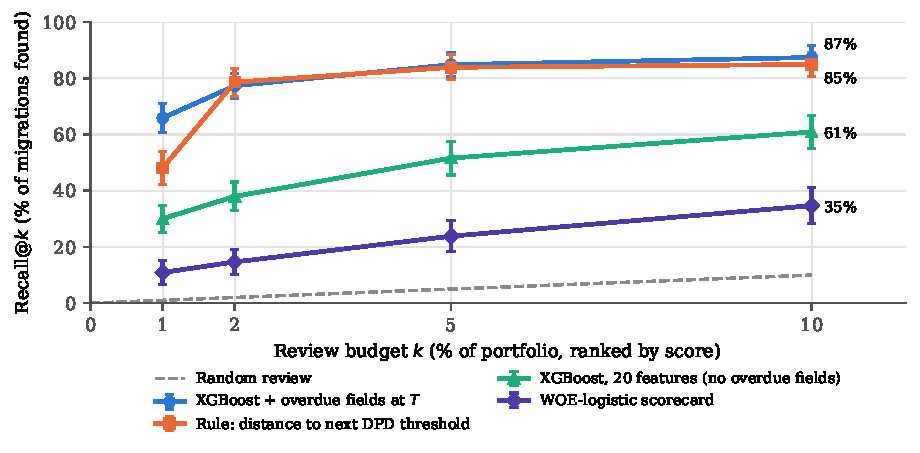
\includegraphics[width=0.86\textwidth]{fig2_recall_at_k.pdf}
\caption{Recall@k (mean $\pm$ sd over 50 folds) by review budget. DPD: days past due; WOE: weight of evidence.}
\label{fig:recall}
\end{figure}

\paragraph{The regulation is a strong baseline.} Ranking by distance to the next DPD threshold, which needs no training, reaches AP 0.203 and finds 84\% of migrations in the top 5\% of the portfolio. XGB on the 20 features does not beat it (AP 0.179; corrected $p=0.45$) and finds only 52\% at 5\%. DPD alone ranks poorly at the top (AP 0.017) because it ignores the group-specific thresholds.

\paragraph{What ML adds.} Adding the four overdue fields at $T$ to XGB doubles AP to 0.393 (corrected $p<0.001$ against the rule), raises Recall@1\% from 48\% to 66\% and NDCG@5\% from 0.48 to 0.56, while Recall@5\% is similar (85\% against 84\%). The gain is therefore precision at the very top of the queue. At a 5\% budget, about 22 loans are reviewed per migration found (Precision@5\% $=0.045$). For the 45 non-mechanical migrations all methods are weak: AP is 0.025--0.033 for the XGB models against a base rate of 0.0005, but with about nine events per fold the fold standard deviations (0.04--0.05) exceed the means, so this signal cannot be distinguished from noise.

\paragraph{Choosing the review budget.} Weighting each migration by the increase in specific provision it triggers (the difference between the rates of Decree 86/2024/ND-CP for the new and the old group times the outstanding balance; all 265 migrating loans are in VND, and amounts are in million VND), the top 1\% of the out-of-fold XGB queue with overdue fields captures 72\% of the total, against 50\% for the rule; at 5\% the shares are 84\% and 67\%. The provision at stake per reviewed loan is about VND 20 million in the top 1\%, but each loan reviewed beyond 5\% adds less than VND 0.5 million. Unless reviews are almost free relative to the provisions they anticipate, a budget between 1\% and 5\% is the defensible choice; the bank's own cost per review fixes the point within this range.

\paragraph{Ranking objective, scorecard and imbalance.} The pairwise learning-to-rank objective is worse than binary classification (AP 0.084 against 0.179, $p<0.001$), as is the WOE scorecard (0.019). Among the six learners on the 20 features (best strategy per learner, i.e., a best-of-strategy estimate; CB was run without resampling only, because of its long run time), XGB without resampling (0.179), LGBM with SMOTE (0.175) and RF (0.167) are statistically tied (Holm-adjusted $p\ge0.42$), whereas a naive Wilcoxon test would separate XGB and RF ($p<0.001$); CB (0.127), DT (0.079) and LR (0.005) are worse. Class weighting raises recall at threshold 0.5 (0.114 to 0.263) but lowers precision (0.911 to 0.072) and AP.

\paragraph{Admissibility and selection sensitivity.} Removing off-balance-sheet interest from XGB on the 20 features leaves AP almost unchanged (0.171 against 0.179, $p=0.23$), unlike Task~1; removing both interest fields lowers it to 0.129 ($p<0.001$), against a random level of 0.0027. For the main model with overdue fields, removing either or both interest fields leaves AP unchanged (0.389 and 0.398 against 0.393; corrected $p\ge0.55$), so its results do not depend on the admissibility of the interest fields. Counting the 45 exits from groups 2--5 as events changes AP only slightly (0.193). In the main model, the most influential inputs by mean absolute SHAP are interest DPD (mean $|\phi|=1.85$), outstanding balance (0.58), actual tenor (0.44), interest rate (0.43) and days to maturity (0.43) (Fig.~\ref{fig:shap}). The largest positive contributions go to loans with short but positive interest DPD, consistent with proximity to the 10-day threshold; the same values could supply reason codes for individual alerts.

\begin{figure}[t]
\centering
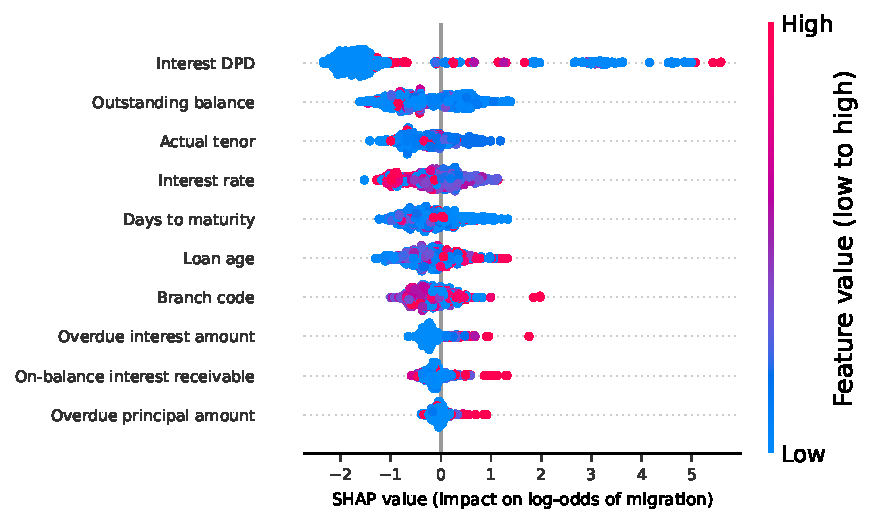
\includegraphics[width=0.66\textwidth]{fig3_shap_beeswarm.pdf}
\caption{SHAP values of the main Task-2 model (XGB with overdue fields) on the label-stratified sample of 53 events and 447 non-events; ten most influential inputs. Colour: feature value (not meaningful for the categorical branch code); DPD: days past due.}
\label{fig:shap}
\end{figure}

% ---------------------------------------------------------------------------
\section{Discussion}
\label{sec:discussion}

\paragraph{Reproducing versus predicting.} The two tasks give different answers to the same question. A five-class model appears strong (Macro-F1 0.69) only because accounting fields restate the label; without them it reaches 0.43, and 0.40 on unseen next-month contracts. A migration model appears useful (AP 0.18), but a rule derived from the classification regulation does as well; ML adds value only once the overdue state at $T$ is given to it, and then mainly by sharpening the top of the review queue. In both tasks, the regulation itself explains much of what the model learns.

\paragraph{Regulation as leakage source and as baseline.} The decisive leakage evidence came from Decree 135/2025/ND-CP rather than from a statistical screen. The most influential leaking field has an IV of about zero, because 93.6\% of its values are zero and decile binning hides its contrast, while the only field above the usual IV alert level is loan age, which reflects seasoning rather than leakage; an IV screen therefore both misses the leaking field and flags an innocent one, and correlation alone cannot establish the direction or timing of a dependence. Likewise, the decisive baseline came from Circular 31/2024/TT-NHNN rather than from another learner. Documenting, for each field, the rule that writes it (Appendix~\ref{app:register}) and benchmarking against the rule that defines the target are inexpensive steps that would change the conclusions of many published evaluations.

\paragraph{Out-of-time evaluation.} Monthly OOT sets mostly contain loans already seen in training, and stable PSI values do not exclude conditional shifts in regulation-produced fields. Pipeline defects can also distort OOT results in either direction: the silent date-encoding change produced a spurious 13--32\% decline, the opposite of the usual optimism bias. Reporting performance on unseen contracts, comparing missing rates and value formats between extracts, and checking how regulation-produced fields relate to the label in each extract should be part of the protocol. For early warning, within-window CV measures ranking quality only inside one window; a deployed model is always applied to a later window, so the regulatory baseline and validation on a later window should be reported next to it.

% ---------------------------------------------------------------------------
\section{Conclusion, Limitations and Future Work}
\label{sec:conclusion}

Using two monthly snapshots of a Vietnamese bank's loan book, this study has shown that (i) a regulation-grounded leakage audit finds a field that inflates five-class Macro-F1 from 0.43 to 0.69 and changes meaning between extracts; (ii) next-month OOT figures overstate transfer because most contracts were seen in training, and silent changes between extracts, such as the date-encoding defect that produced a spurious 13--32\% decline, can distort them in either direction; and (iii) most 31-day migrations follow the regulation's DPD thresholds, so a rule-based ranking is a strong baseline that ML beats only when given the overdue state at prediction time, mainly at the top of the review queue.

Two limitations are most important. First, the evidence comes from one bank and one 31-day window with 265 events, of which only 45 are non-mechanical. Whether the strength of the regulatory baseline and the ML gain persist in later periods and over longer horizons (3, 6 and 12 months) is untested and must be verified on further snapshots; a model fitted on one window should be validated on the next before it is used. Second, the admissibility of the interest and overdue fields at $T$ assumes that they are not revised retroactively, which should be confirmed with the bank; and the bank could not provide reason codes for contract exits, so exits from groups 2--5 are handled only through the sensitivity analysis above. Future work will compare these results with the approaches of~\cite{nguyen2025boosting,nguyen2024ews} on the same data, extend the evaluation to further monthly windows and longer horizons, and fix the review budget within the 1--5\% range using the bank's actual cost per review.

\paragraph{Data availability.} The loan-level data are proprietary, were provided under an academic research arrangement and cannot be shared. The code that reproduces all tables and figures from the stored results is available from the corresponding author upon reasonable request.

\paragraph{Disclosure of interests.} The authors have no competing interests to declare that are relevant to the content of this article.

\paragraph{Acknowledgements.} The authors thank the partner bank for providing access to the data. None of the models developed in this study was used for lending decisions.

\appendix

\section{Field Register of the Leakage Audit}
\label{app:register}

\begin{table}[h]
\centering
\caption{All 33 fields of the reporting template and their treatment.}
\label{tab:register}
\scriptsize
\begin{tabular}{@{}>{\raggedright\arraybackslash}p{2.6cm}>{\raggedright\arraybackslash}p{6.6cm}>{\raggedright\arraybackslash}p{2.4cm}@{}}
\toprule
Treatment & Fields & Basis\\
\midrule
Target (1) & Self-assessed debt group & Circular 31/2024\\
Excluded, Layer 1 (7) & CIC-reconciled debt group; overdue principal amount; principal overdue date; overdue interest amount; interest overdue date; specific provision required; specific provision booked & Alternative label; DPD thresholds; Decree 86/2024. Overdue fields used at $T$ in Task~2\\
Excluded, Layer 2 (6) & Customer identifier; customer name; credit agreement number; contract number (join key); recovery date; paid amount & Identifier; duplicate of contract end date; constant zero\\
Used to engineer features (3) & Reporting (ETL) date; disbursement date; contract end date & Loan age, days to maturity, actual tenor\\
Retained, Layer 3 (2) & On-balance-sheet interest receivable; off-balance-sheet unpaid interest & Decree 135/2025, Art.~13(2)(a); excluded from main Task-1 results\\
Retained (14) & Branch code; interest rate; outstanding balance; number of restructurings; restructured principal; restructured interest; electronic-channel flag; credit term code; credit form; lending method; currency code; purpose by economic sector; purpose description; funding source & Contractual or balance attributes at the reporting date\\
\bottomrule
\end{tabular}
\end{table}

% ---------------------------------------------------------------------------
\bibliographystyle{splncs04}
\bibliography{references}
\end{document}
